\documentclass[12pt]{article}
\usepackage{xcolor}
%\usepackage[tmargin=1in,bmargin=1in,lmargin=1.25in,rmargin=1.25in]{geometry}

\usepackage{geometry} % Required to change the page size to A4
\geometry{a4paper} % Set the page size to be A4 as opposed to the default US Letter

\usepackage{graphicx} % Required for including pictures
\graphicspath{ {diagrams/} }

\usepackage{float} % Allows putting an [H] in \begin{figure} to specify the exact location of the figure
\usepackage{wrapfig} % Allows in-line images such as the example fish picture
\usepackage{psfrag,amsmath,amsfonts,amsthm,amssymb}
\usepackage{lipsum} % Used for inserting dummy 'Lorem ipsum' text into the template
\usepackage{listings} %for inline code

\linespread{1.2} % Line spacing



\usepackage{setspace}
	\onehalfspacing

\usepackage{biblatex}
	\bibliography{mqp_bib.bib}


\usepackage[draft]{todonotes}

\usepackage{hyperref}
\usepackage{mathtools}
\usepackage{algpseudocode}
\usepackage{algorithmicx}

\newcommand{\comment}[1]
{{\bfseries \color{blue} #1}}

%a lazy citation placeholder.
\newcommand{\lcite}[1]
{{\bfseries\color{orange}[#1]}}

\newcommand{\prettycode}[1]
{\lstinline[basicstyle=\ttfamily]{#1}}



\begin{document}

\title{Bandwidth Aggregation Over The HTTP Protocol}
\author{Dan Robertson}
\date{April 2014}
\maketitle

\begin{abstract}
	Computer networking often pushes the limit of available bandwidth. Although bandwidth speed has historically increased 10 fold in recent years, newer and faster speeds often come with a steep price increase. Moreover, the failure of one high speed link results in a significant drop in a network's instantaneous bandwidth. Luckily, a more clever, cost efficient solution to this problem already exists. Bandwidth aggregation allows multiple network links to be combined into one logical interface with the combined bandwidth of the supporting links. This comes with the benefit of fail over redundancy, allowing the network to adapt and recover from link failures. This has been achieved at the lowest 3 layers of the OSI model, with both proprietary and open software solutions in existence that get the job done.But it has yet to become pervasive in growing WIFI and WAN networks. Many implementations at this level have been proposed (such as Multipath TCP), but few are realizable by the typical consumer.

	This MQP proposes a new method for bandwidth aggregation, utilize-able by the typical home network owner. The methods explained herein aggregate a network of coordinating routers within local WIFI communication range to achieve increased bandwidth at the application layer, over the HTTP protocol. Our protocol guarantees content delivery and reliability, as well as repudiation measures that hold each participant, rather then the group of routers, accountable for the content they download.
\end{abstract}


\newpage
\section{Intro}

	%introduce NABC, explain the approach briefly, mention the results, include organizational remarks at the end
	An influx of bandwidth intensive services over the past decade has placed an increased demand for high speed connections on the shoulders of Internet Service Providers (ISPs). However, the demand is overwhelming to the typical ISP, who has to enforce a fair and steady bandwidth between each subscriber in order to keep their network healthy. It is now common place that ISPs apply traffic shaping rules, in order to enforce an upper limit on bandwidth alloted to each client. Cellular service providers, who employ long distance wireless communication channels (such as LTE) to guarantee Internet coverage to mobile clients, rate limit their clients for the same reasons. 

	It is often the case that clients (both mobile users and home owners) naturally cluster together in close proximity (by nature of our society). One can imagine the number of mobile devices crowded together at a busy bus stop, or the overlap of routers (each with a separate ISP subscription) within wireless communication range of each other in a city apartment. Combining these rate limited neighboring devices can yield download speeds that comes close to the true sum of the parts. This very idea has become a low hanging fruit in the networking community. This has lead to a surge of academic works which empirically guarantee bandwidth aggregation at various layers of the OSI model. However, very few are found in practice today, and even fewer are practical to the consumer. A great number of works have focused on aggregating the bandwidth of LTE users into altruistic communities, which offer higher bandwidth then that of an individual link. However, in the apartment setting, only a limited number of commercial offerings have been devised. This MQP seeks to contribute to the latter case. 

	Existing bandwidth aggregating solutions available to consumers have two shortcomings. Their functioning requires the presence of a special router (for each client), and they fail to provide strong security guarantees. Our approach leverages the HTTP protocol in order to aggregate bandwidth between a number of routers, called {\it peers}, in local wireless range of each other. This means that our solution is inherently protocol dependent. However, since the majority of web traffic is carried across HTTP, it is prevalent enough for most use cases. It can be run on any Linux platform (such as the DD-WRT router firmware), making home installation an easily achievable reality. Our solution comes in the form of an HTTP proxy server, targeted to run on a router, which acts as an intermediary between the client and the router its self. It can be thought of as the brain behind the aggregation schema, letting the router handle the transport of all traffic without having to worry about the mechanisms being used for aggregation. Further, it safeguards participants from being incriminated for traffic they unwillingly download on behalf of other peers, through strict enforcement of non-repudiation. This guarantees that participants in a proxy community can not be held accountable for traffic they ferry on behalf of neighboring participants. 

<<<<<<< Updated upstream
	Our bandwidth aggregation protocol was implemented in Python, and tested on both real and virtualized hardware, with the majority of our data coming from the controlled virtualized environment. We found that the bandwidth realized by the client is close to that of the summed bandwidth of each involved router. 

	The report is organized as follows. Section 2 provides an extensive overview of the current bandwidth aggregation client, beginning with its inception in the late 1990s, up to the modern trends of the past decade. Our initial approach to implementing the proxy, and explanation of our design rationale is given in section 3. Detailed results of our evaluations, and an overview of the process, can be found in section 4. Discussion on the various cryptographic primitives and security protocols adapted for use in this proxy, such as non-repudiation, trust factors, and signature verification using a public key infrastructure, can be found in section 5. Related works, and suggested areas for future improvements to our approach, can be found in section 6.
=======
	Our procedure and software were tested on both real and virtualized hardware, with the majority of our data coming from the controlled virtualized environment.\comment{Talk more about end results, once they are confirmed}

	The report is organized as follow. Section 2 provides an extensive overview of the current bandwidth aggregation client, beginning with its inception in the late 1990s, up to the modern trends of the past decade. Our initial approach to implementing the proxy, and explanation of our design rationale is given in section 3. Detailed results of our evaluations, and an overview of the process, can be found in section 4. Discussion on the various cryptographic primitives and security protocols adapted for use in this proxy, such as non-repudiation, trust factors, and signature verification using a public key infrastructure, can be found in section 5. Related works, and suggested areas for future improvements to our approach, can be found in section 6.
>>>>>>> Stashed changes




%=====================HISTORY=================================================%
\newpage
\section{Background}

	The practice of link aggregation was first defined in the 802.3-2000 IEEE standard. It came as a continuation of the work started by a task force that the 802 group assembled on November of 1997, to address the then disparate trend of link aggregation \lcite{802 trunking tutorial}. They recognized that Ethernet was most of the market, and that several vendors already had solutions for aggregating existing physical links to provide a faster Ethernet connection. However, an inter-operable solution was desired. The protocol they developed became known as the ``Link Aggregation Control Protocol''(LACP), officially as 802.3ad, but later moved to 802.1ax \lcite{IEEE 802.1ax}. LACP provides a reliable mechanism for aggregating Ethernet links which implement the same protocol. It allows for the controlled addition and removal of links from an aggregation group without disrupting the stream of data frames \lcite{IBM IEEE}.

	One of the core principles behind link aggregation, and this MQP, is cost. Upgrading to a higher speed link is always an option, but trunking together multiple existing lower speed links can satisfy most, if not all, of the same needs. This also provides resilience, since a failure of one link just means a decrease in throughput, instead of a total loss, as LACP will automatically load balances between the remaining available links. LACP works great for enterprise network operators who have access to the necessary physical links and switches, but has a few short comings. LACP is inherently targeted for neighboring physical connections, which can only be combined through use of additional hardware (namely, a switch). These shortcoming would become more apparent as demand for high bandwidth wireless LAN and WWAN grew.



\subsection{Heterogeneous Wireless Networks}

%===============HETEROGENOUS WIRELESS=====================================%
	With the surging popularity of video streaming, high definition media, and online gaming, bandwidth limits have again become a problem for residential addresses. Multinode terminal devices (such as smart phones) have the power to actively switch between Radio Access Technologies (RATs), but few actively use this technique. Aggregating several RATs, such as LTE and WiFi, would give these devices better fail over redundancy and increased bandwidth.

	Ramaboli et al. present a comprehensive review of the current climate of bandwidth aggregation in heterogeneous wireless networks. They identify a number of common concerns that various bandwidth aggregation techniques must address in order to be proficient. Amongst these issues is packet reordering, which becomes necessary in any situation when items are delivered out of order. This erupts from the inherent invariability of link conditions within the Internet. Any response that travels over different paths will each be subject to differing latencies and delays. It is an unavoidable consequence of aggregating two seperate streams. This introduces a buffer overhead into the session, which must be absolved by the client, server, or any intermediary hops along the way (depending on the architecture of the particular approach)\cite{Ramaboli20121674}. The second issue, battery power, becomes more of an issue on free roaming mobile devices which aren't constantly tethered to a power source. This MQP effectively sidesteps this battery power issue by performing all aggregation logic on a persistently powered device.

	A tenet of successful bandwidth aggregation is the preservation of packet order. Combining multiple RATs can yield throughput equivalent to the sum of the individual lines. This helps reduce load on a particular link by evenly distributing it over many links, so long as the distribution order preserves packet order. Packet reordering does not just bloat buffer space, or slow down reassembly at the client end. Packet reordering outside a certain sequence range will trigger a TCP loss event, which shrinks the transmission window and negatively affects throughput, leading to an underutilization of the aggregate bandwidth capacity\cite{Ramaboli20121674}.

	Jayasumana et al. suggest a set of metrics to help evaluate packet reordering, these are Reorder Density (RD) and Reorder Buffer-occupancy Density (RBD). Reorder Density describes the distribution of out of order packets (normalized to the number of packets) for any given sequence. Reorder Buffer-occupancy Density measures the buffer occupancy frequencies normalized to the number of non duplicate packets. This metric can be good for predicting the amount of resources required to perform packet reordering\lcite{RFC5236}.

	Ramaboli et al. conclude that all wireless bandwidth aggregation techniques can be pigeonholed into one of two slots, based on how they attempt to circumvent the need for packet reordering. Adaptive bandwidth aggregation observes various link conditions in order to smartly route packets of varying size between interfaces. This would obviously be the preferred method, as it lowers the chances of out of order delivery. Non-adaptive bandwidth aggregation uses static link selection (such as round robin) in order to route sub-flows. This can lead to lower throughput when link and traffic conditions are not constant (as a result of factors such as jitter)\cite{Ramaboli20121674}.

	Bandwidth aggregation has been realized on all network layers except the physical. The numerous methods at each layer vary significantly in their levels of transparency, administrative overhead, and infrastructure leverage. Each must implement two basic methods; one to divide traffic over multiple links, and one to reassemble the traffic.

	\subsection{Application Layer}

		Solutions at the application layer have access to multiple outgoing interfaces, and can split the data into several application layer chunks (as this MQP does with HTTP) which can then be transmitted simultaneously over these interfaces. However, the aggregation must be application specific, and does not provide more general, application agnostic aggregation. Examples include XFTP, MuniSockets and parallel sockets. XFTP and Parallel Sockets both maintain multiple TCP connections over a single interface to any number of distributed servers\cite{Ramaboli20121674}. Multiple TCP protocols (\cite{1541208}, \cite{4539690}) leverage the idea of parallel sockets for downloading file portions from distributed servers. This technique alleviates load on a target server, by spreading requests out to multiple sister servers (who are assumed to have the same requested resource). They achieve similar goals to bandwidth aggregation by providing failover redundancy, recovering from server failure by off putting the remained of the download to another target. Note that while these methods do not aggregate multiple network interfaces, they do share some common ground with this MQP through their technique of parallel segmented downloading.

		Mohamed et al. propose Multiple Network Interface Sockets (MuniSockets), a protocol which performs true aggregation of multiple physical interfaces, maintaining a separate thread for each connection, on both the client and server end. A counter is used to compute sequence numbers for each data chunk. Each chunk awaits a vacancy in the send buffer before it is sent out. Naturally, chunks may arrive out of order at the receiver. MuniSockets holds these chunks in a reorder buffer until they can be properly spliced into the data passed back to the client. It uses selective acknowledgments (in a vain similar to that of TCP) to deal with retransmissions. Unfortunately, it assumes static, unchanging network conditions, and thus does not respond to jitter or delays\cite{mohamed2002user}.

		As application layer solutions isolate modifications to the most infrastructure independent layer, they are more realizable in the short term. Although modification at the client and server is a demanding requirement of application layer solutions, they are available to end users who are motivated to upgrade. Solutions at other layers tend to require infrastructure changes on a far wider scale. Due to the ossified nature of the Internet, realizing most lower layer solutions on a wide scale is an ambitious and difficult endeavor.

	\subsubsection{Transport Layer}

		Transport layer bandwidth aggregation solutions do not require application or network layer modifications, provides path transparent congestion control, and have experienced a surge in research over the past decade\cite{5763587}. However, TCP is not inherently optimized for timely delivery, so using it as a mechanism for aggregation only provides so much gain. Popular streaming services, which are fairly bandwidth intensive, such as Netflix and Spotify, use UDP and can't be remedied by TCP protocol modifications.

		Multipath TCP (MTCP) has been defined by the IETF in 2011. It extends the TCP protocol to support multi-homed endpoints (a multi-homed client has multiple IP addresses). A Linux Kernel implementation of MPTCP has been developed and is currently undergoing community experimentation, as its popularity grows \cite{barre2011multipath}. Apple caused a spike in interest in MPTCP by subtly building it into their iOS7 software.\footnote{Their technical documentation does not advertise their use of MPTCP, but WireShark captures reveal that iOS7 sends MPTCP specific requests under certain use cases.} While it is only used for their Siri service in order to provide smooth Internet access when one RAT unexpectedly cuts out, it represents the first commercial adoption of the protocol.

		Multipath TCP works by breaking outgoing data from the application layer into multiple streams that can travel out different interfaces. The MPTCP stack on the host communicates each available peer address at its disposal to the server, with each address denoting a unidirectional path to the instance. It also handles separating each TCP subflow out and gluing returning data from these flows back together, so they can be delivered to the application. Across the network, these subflows are just typical TCP connections, which are handled by each hop as they would normally. This transparency enables MPTCP to work in any situation which traditional TCP would have worked\lcite{MPTCP netys}.

		Stream Control Transmission Protocol (SCTP), provides multi-homing out of the box. Out of the box, it only uses one stream (the primary path) per transport direction, instead of one stream for both (as in TCP). All other available streams are used when the primary path fails. The collection of SCTP streams are denoted as an {\it Association}, and data packets sent over them are divided into chunks, which may be delivered out of order. The SCTP stack on either end then handles reordering these packets. SCTP enforces a congestion control window similar to TCP's over each path, and mimics many of TCP's default functionality over each of its streams\cite{5763587}. While this isn't a gleaming case of multi-homing, it provides a framework for experimental work. Many SCTP variants achieve bandwidth aggregation, some of which are described in our overview of adaptive bandwidth aggregation solutions.

	\subsubsection{Network Layer Solutions}

		Network layer bandwidth aggregation solutions yield a much desired transparency to upper layers. Unfortunately, it is prone to out of sequence arrivals, which must be dealt with while consuming as little buffer space as possible.

		The Round Robin packet scheduling algorithm, which runs in O(1) time, is a simple preexisting network layer approach to bandwidth aggregation. Packets (assumed to be of the same size) from the same flow are assigned to multiple paths in a circular matter. The RR scheduler only works so well in theory because it assumes homogeneous packet size and transmission rate. This is very rarely the case however, so the approach falls short. In realistic scenarios, the round robin approach to scheduling may limit the effective bandwidth to that of the slowest path.%find citation%

		Kim et al. (2008) proposed a BA scheme that employs two metrics for scheduling; bandwidth estimation and packet partition scheduling. The former determines the amount of bytes that can safely be transmitted across a link without triggering congestion. The latter decides how packets can be assigned to different paths in order to effectively balance load. A partition counter is assigned to each path, which is used to determine whether the associated path can accommodate a new packet\cite{kim2008packet}.

		Evensen et al. introduce a method that uses network stripping, a process which splits traffic over multiple different links, in order to aggregate bandwidth for multihomed clients. In order to minimize reordering at the client, they employ a smart proxy to buffer out of order deliveries, and delegate packets to different interfaces. The proxy acts as both a scheduler and delay equalizer. It decides which links to send traffic through based off of observed throughput. The delay equalizer is used to mitigate client side reordering, by delaying packet retransmission\cite{5355198}.

	\subsubsection{Data link Layer}
		The data link layer was where earlier solutions to bandwidth aggregation lived. It was not until the mobile network boom that attempts to aggregate heterogeneous RATs at the link layer began again. One such realization of this practice is the Generic Link Layer (GLL) protocol. GLL is a multi access radio architecture that aims to unite differing RATs under a transparent session. GLL allows for Multi Radio Transmission Diversity.
		\begin{quote}
			MRTD is defined as the data flow split (on IP or MAC PDU level) between two communicating entities over more than one RAT. This comprises parallel transmission, or dynamic switching between the available RATs.\cite{GLL:2005}
		\end{quote}
		MRTD can select its links based off criteria such as traffic requirements and estimated link quality. However, like many others, this approach to bandwidth aggregation struggles with the issues of packet reordering and unbalanced load distribution\cite{Ramaboli20121674}.

\subsection{Adaptive bandwidth aggregation}

	The pitfalls of the na\"{i}ve approach (non-adaptive bandwidth aggregation) manifest themselves at every layer. Static decision making for link selection ultimately lead to out of order delivery of differing data segments, which must then be addressed by packet reordering. Adaptive bandwidth aggregation considers the varying link and traffic conditions when organizing sub-flows between multiple interfaces. A variety of these approaches exist, of which Ramboli et al. provide an excellent overview. 

	At the application layer, Luo et al. \cite{1204756} split traffic into important and non-important stream, delivering each stream over a different RAT. Protocols such as HTTP, which mix important main page objects with unimportant inline objects (such as photos and advertisements), benefit greatly from this dissection. A small training packet is sent along each link to calculate the RTT and delays, this is done intermittently and allows their implementation to better split traffic between different links. Splitting traffic into streams is often done with video content, where a base layer (necessary for decoding the video) is separated from different high level enhancement layers, which enrich viewing of the video. Each of these streams are sent over different channels, with the lower layers (starting with the base layer) receiving higher priority. Here, the base layer is assigned to the most reliable path, ensuing layers are assigned to the remaining available paths based on their priorities\cite{1363842}.

	Multimedia data transfer over multiple access channels is explored by Kasper et. al, in an attempt to asses the improvements to video-on-demand playback given by bandwidth aggregation. They note that startup latency (the waiting time before the video can begin) and large buffer overheads are amongst the greatest challenges in progressive downloading over multiple channels. Accordingly, segment size plays a key role in determining the extent of these challenges. The larger the segment size, the bigger the buffer requirements. They identify that the number of network interfaces used as part of aggregation also increase the buffer requirement. It then becomes an issue of algorithmically determining the optimal segment size, in order to minimize startup latency and buffer requirements\cite{5421846}.

	W-SCTP, an extension of the stream control protocol, uses a bandwidth aware scheduler (implemented on the sending end) to manage subflows across multiple paths [Casetti and Gaiotto (2004)]. It maintains separate send buffers per interface, and sends each segment down the fastest one until each path has reached its congestion window limit. This approach does not deal with segment reordering, and fails to use the vast majority of metrics\comment{explain} for optimal link selection. 

	Also see LS-SCTP, which achieves one logical congestion window made up of the aggregate of the participating paths. Flow control is separated from congestion control, allowing each path to have its own congestion window, while flow control logic happens by association with the session. Data is broken into chunks and assigned to the best path based on continuously measured channel statistics (such as bandwidth). The congestion window is closely monitored in order to determine which path to send a particular chunk across\cite{AbdElAl20041012}.

	Arrival time matching load balancing (ATLB) [Hasegawa et al. (2005)], presents a solution to the ordering problem. ATLB scores each path by end-to-end delay, and uses this heuristic (lower is better) to assign each segment to a path. This significantly cuts down on out of order delivery, but a reorder buffer at the client is still maintained to deal with infrequent reordering issues.

\subsection{Mobile Devices as an Aggregation Platform}

	Multi-homed mobile devices (most prominently smartphones), offer a low hanging opportunity for bandwidth aggregation. With the typical person carrying one active mobile device on them at all times, the potential to treat each device as a hand held router opens up an exciting array of possibilities for intelligent and dynamic bandwidth aggregation. Typically, a bandwidth pool between client devices is achieved through inverse multiplexing. The challenges of this set up come from the ephemeral nature of the participating community members. A mobile user may enter a bus with dozens of other users, where a community may or may not already exist. Another user may exit at the next stop, and the community would have to adapt to the sudden loss.

	Sharma et. al simulate these ideas in order to justify future research in collaborative bandwidth aggregation for mobile systems. They devise a system in which mobile peers dynamically form ad hoc {\it Mobile Collaborative Communities}, in which each member creates a communication channel to the inverse multiplexer (optimally a proxy), which can then be used (partially or in full) by other members of the community. The summation of these channels can be logically combined by an inverse multiplexing protocol in order to offer one logical high speed aggregate channel\cite{1363842}. Their simulations show that bandwidth increases linearly with each added participant to the pool\cite{1363842}.


\subsection{Non Repudiation, and Willingness to Participate}

	Sharma et. al pose the question: do mobile users desire to share their personal communication channels (in a utilitarian fashion)? Once the question of how to aggregate has been thoroughly solved, the end user still has to agree to participate. This is especially the case when aggregation hinges on the participation of a client's own device (such as a mobile phone, laptop, or router). Fortunately, user bandwidth is low cost, and users can volunteer as little as they desire. A good protocol should prioritize individual user experience, so that one peer can never interfere with the quality of service of another peer. \cite{1363842} optimistically looks at the the success of peer to peer services, inferring that users who are willing to share their data will also be readily willing to share their communication resources. However, there is one final threat that users should not have to worry about; accountability. There must be a system in place to ensure that a peer cannot be prosecuted for blindly passing along malicious or illegal traffic that enters the pool.

	Non-repudiation allows us to provide this guarantee. It facilitates liability and thus self accountability by guaranteeing indeniability for any particular interaction. This can be more clearly illustrated through a message exchange between Alice and Bob, a quintessential cryptographic metaphor for a sender/receiver. If Alice sends a message to Bob, who receives it, neither Alice or Bob should be able to deny their transmission / receipt of the message (respectively). This introduces the notion of fairness to non-repudiation. In our example, Alice would maintain a non-repudiation of origin record (proving that she was in fact the sender), and Bob would hold a non-repudiation of receipt record (proving that he did indeed receive the message). This essentially guarantees that one party cannot fool the other\cite{Kremer20021606}.



\section{Approach}

	A detailed assessment and overview of the optimal design for an HTTP bandwidth aggregating proxy is given in the proceeding section. A proof of concept python implementation was designed in parallel with the writing of the paper. This implementation has been stripped of some of the auxillery features described herein, but works as an excellent foundation which could be extended to accomplish all of them.

	\subsection{Core Design Components}

		\subsubsection{Determining when to aggregate}

			Certainly, not all Internet traffic merits bandwidth aggregation. A typical web request, be it for a JavaScript library or page markup, rarely exceeds the double digit range in kilobytes. The small overhead given by the inter-router communication needed for our protocol outweighs the download time of the small packet. A na\"{i}ve approach would be to find the response size for every packet, and judge based on that. The HTTP protocol provides us with a way to do this, using the HEAD method, which asks the server for only the headers (including content-length) of the target resource. These requests are very small in size, but still suffer from an end to end delay between the client and server. Since today's web pages often require dozens of resources to be fetched from various locations before a page can be completely displayed, many HTTP HEAD requests would have to be made, on top of the standard GET request (used to retrieve the data) in order to load a single page. For a large number of small requests, the round trip delay of sending a HEAD request for every packet introduces an unfavorable latency for typical web sessions. 

			Our solution was to issue all requests in a normal manner, without trying to ascertain whether or not bandwidth aggregation was necessary before passing the request to the server. When a response comes back, the content-length header is always specified, which gives us a better clue of the size of the impending response. If the dictated size is over a certain threshold, the connection is terminated and the same request is issued again, this time in the context of our bandwidth aggregation scheme.

		\subsubsection{Negotiating Peer Involvement}

			Our protocol works by mustering a garrison of neighboring routers (neighboring herein will be used interchangeably with peers, and will refer to network devices within wireless range of each other who are capable of running our software) to farm aggregation out to. In order for a peer to participate, it must be within wireless signal range of the initiating router, where the connection between the two is consistent and unlikely to cut out. This brings to mind the notion of reliability. The peer must be capable of providing the services requested in a timely manner. Peers who frequently timeout or drop requests mid session are considered to be unreliable. This measure requires a good amount of auditing and record keeping to be done by each router.

			Optimally, each peer router would determine how much of it's total bandwidth it can commit to the session. If a download session would negatively effect the Quality of Service the router provides to its own client, then it should opt out of the session. The idea behind this is to maximize unused bandwidth, while still guaranteeing the normal amount available to each individual router. Our implementation was developed as a proof of concept, and does not support this bandwidth estimation functionality. It is there fore left as a suggestion for future work.

		\subsubsection{Security and Liability}

			Our schema utilizes multiple neighboring routers to download differing sections of the same resource. Further down the Internet pipe, an observer would perceive each neighbor as requesting the same source. Therefore, any illegal traffic downloaded using aggregation can potentially be traced back to the owners of each participating router. This risk must be understood by each participating user. To combat this concern, our protocol guarantees non-repudiation, eg. an aggregation session can always be traced back to the originator. This is achieved using digital signatures for each session, using a trusted third party, and is explained in further detail in our discussion.

		\subsubsection{Request Segmentation and Distribution}

			This MQP proposes two methods for request division and segmentation. The first is an adaptive solution, which requires peers to keep track of their own bandwidth utilization at any given time. When requesting peers for help in a download session, a peer will respond with the bandwidth they can offer at the time of the request. The peer would then be given a localized chunk size that is derived from their advertised bandwidth and the size of the file. In an ideal situation, each peer would finish their section in a similar interval. The non adaptive solution assigns fixed size chunks to each router in a round robin fashion, never delegating more then $n$ chunks at a time (to safeguard against buffer bloat) before the first chunk has been received and sent. In this approach, chunk size quickly becomes an issue. The amount of buffer space and memory on the device will play a key role in determining this. On embedded devices, such as traditional routers, the buffer cannot be to big.


	\subsection{Deciding on a Device}
		
		Originally, we focused our methodology on adopting a single device to implement a platform specific aggregation solution on. Later, we extended our implementation to run on any network capable device that can run python, as we wanted this to be achievable by any home network owner.

		We narrowed down the scope of our device search to three major families of devices: routers, single-board computers, and traditional desktop computers running  Linux. The first of the single-board family is the Raspberry Pi. Small, cheap, and robust, with a personalized flavor of Linux and support for just about any framework desired, the Pi was an attractive choice. It can be modified to meet a wide variety of needs, one of which includes emulating a router. The Pi can supports a growing number of programming languages and boasts 2 GB of free disk space on the cheapest model. However, with a limited number of outgoing ports (2 USB and 1 Ethernet), the quality of router this device could mimic is not so favorable.

		Second, a conventional Linux box could have been used. There is a large variety of network purposed Linux distributions and debian derivatives of various capabilities, which could be installed on any Linux platform. This could enable us to use multiple network interfaces and a powerful CPU with plenty of memory, which could perform well as router. This flexibility makes the combination of a robust distro and powerful hardware a hard option to ignore. However, the catch is the gluttony of the machine, as well as the deployment cost, if an existing device was not available. Although the goal of this project is to provide a proof of concept prototype for our model of bandwidth aggregation, a cost effective implementation would be beneficial. 

		The third possibility was to use an existing wireless router and flash it with open firmware that would allow it to be more easily altered. The configuration options provided by a commercial router out of the box would not allow for low level modification, and bandwidth aggregation cannot simply be achieved through altering a few NAT tables, so firmware replacement was a necessity. Because of an oversight of the GNU public license, Linksys developers were force to make their WRT-54G drivers completely public in order to comply with the license. This opened up the door for a variety of hacked WRT firmware variants to be developed, eventually leading to DD-WRT. A large variety of common commercially available routers can run this firmware.

		DD-WRT is a popular implementation amongst do-it-yourself networking enthusiast. It provides a large amount of functionality not present on the original router firmware, most of which is exposed in its configuration options\lcite{DDWRT homepage}. While the added functionality was nice, what we were more concerned with was the ability to load and run custom applications onto the router. For this, OpenWRT (a cousin of DD-WRT) seemed like a better solution. 

		OpenWRT functions similar to DD-WRT, but it has more developer support and a livelier community then that of the DD-WRT. It comes preloaded with a package manager that makes installing custom software easy, which allows for the creation of C/Python packages and even Kernel Modules. These add-ons can be flashed onto the router as executables, or bundled with the original firmware image. 

		After reviewing all the device choices, we decided to use OpenWRT for the project. Implementing router to router bandwidth aggregation on a router seemed to be the most straightforward option. But as the project evolved, it became clear that a router implementation was an end goal, the software which we were to write could function better on a higher power Linux machine with multiple network interfaces and plentiful amounts of memory and disk space. The trick was to implement a software solution that was largely device independent, using an interpreted language such as Python. This would allow end users to run the software on their choice of Python capable hardware, be it a flashed router, Linux computer, or Raspberry Pi.

	\subsection{First Design Iteration}
		
		After choosing to implement the project on routers flashed with OpenWRT, we began to map out the technical implementation. Our approach would evolve over time as I researched the capabilities and limitations of the chosen platform. 

		{\bf High level overview of our idea}
		\begin{itemize}
			\item[1] A daemon will run on each router, that monitors traffic coming through the router, and will decide (based on some selection algorithm) whether or not to perform bandwidth aggregation for the request
			\item[2] The router will ask neighboring routers to participate in an aggregation session for the specified request
			\item[3] The initiating router will then divide the request into a number of chunks, and hand them to each neighbor.
			\item[4] Each neighbor will download the chunk, and forward the response data to the initiating router, who will send it to the client.
		\end{itemize}

		Our first hurdle was to figure out how to make the routers exchange data to and from the server, in a way that preserves the router's credentials. For instance, if router A sends a packet to router B that is meant for the server that the host originally requested a file from, B would not know the address of the server, as B only sees the source address from A, and the destination address as its own. We quickly realized that encapsulation was needed. 

		\begin{figure}[H]
			\centering
			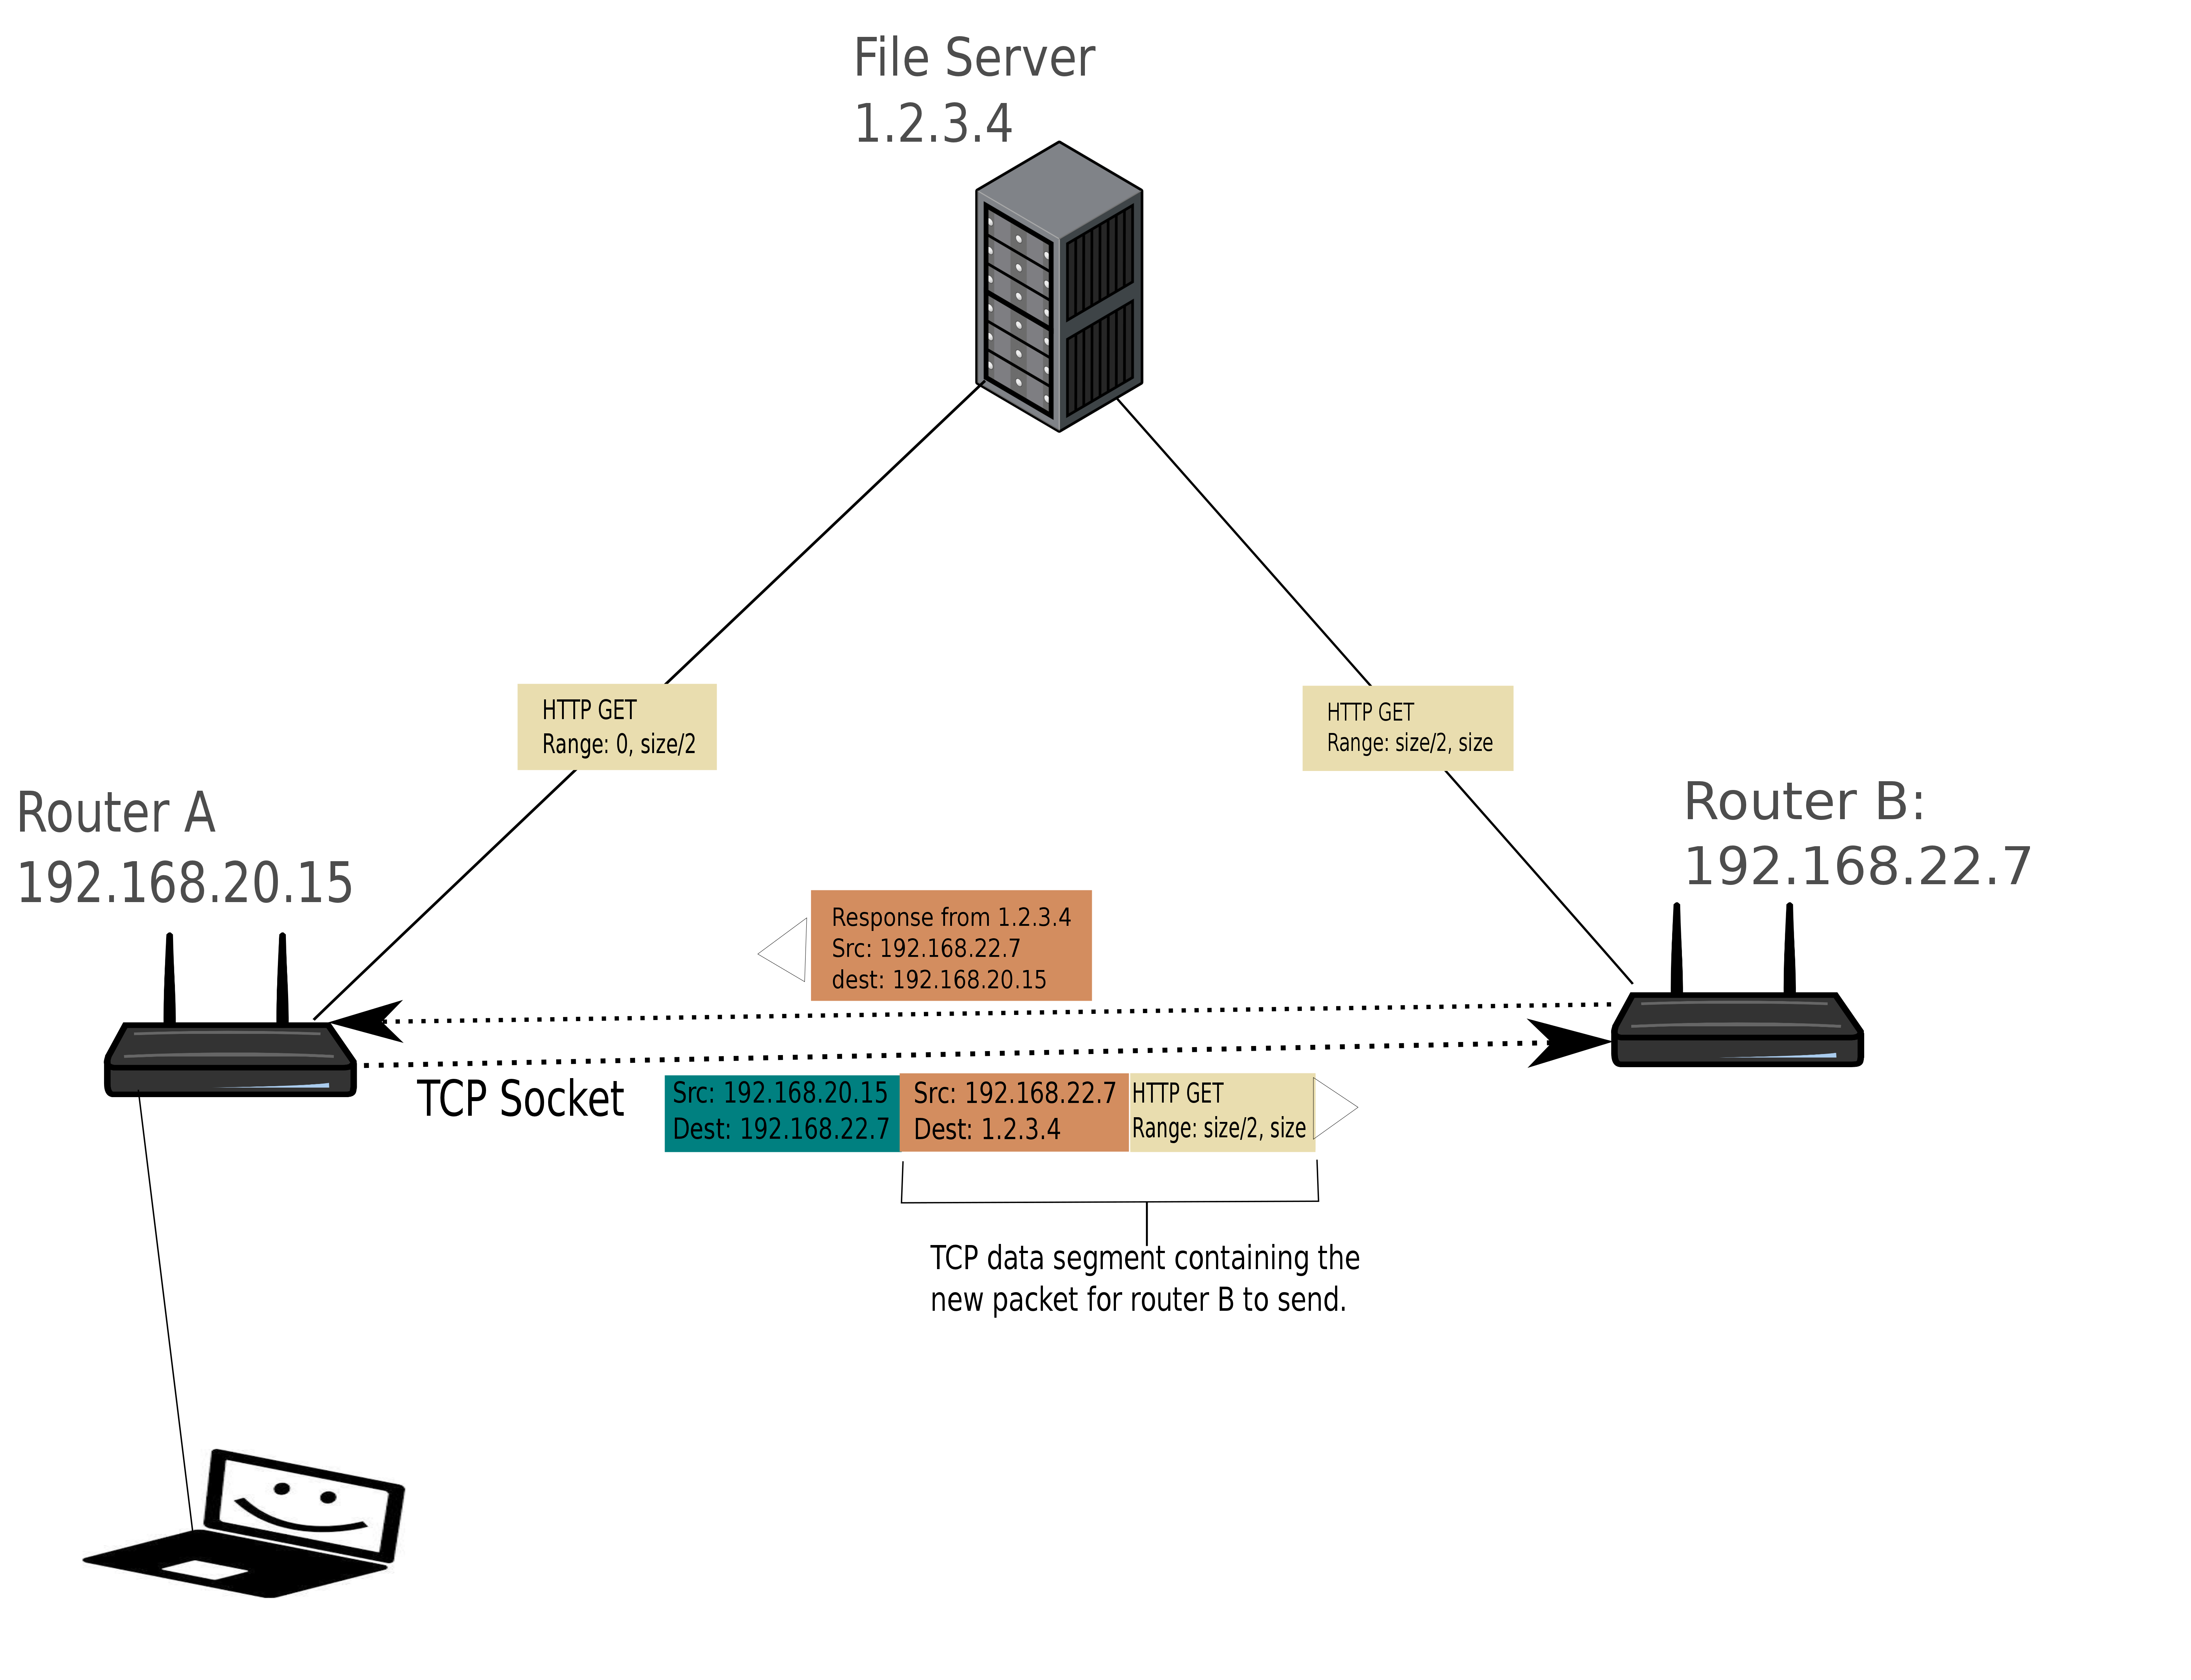
\includegraphics[keepaspectratio=true,scale=0.08]{RouterDiagram.png}
			\caption{Initial plan for router to router communication, using encapsulation and NAT.}
		\end{figure}

		Because the two routers need to exchange information freely, we would have to open a TCP connection between both routers. This connection would be set up when a router agreed to participate in an aggregation session. The initiating router would then send request information (URL of server, the size of the file) to the participating router, who would then issue its own request to the destination. The participating router would then set up a mapping, perhaps using Network Address Translation, to forward the responses it gets from the server back to the initiating router, which would then deal with the data accordingly. Eventually, we came to a model similar to this

		This lower level approach had a number of pitfalls which promised to be a significant hurdle for the implementation of the software. It became apparent that the core firmware of the router would have to be modified in order to achieve certain goals. Even the flexibility granted by Open-WRT would not be sufficient enough to permit per packet inspection and decision making. The issue was that we were trying to make routers do something outside of their original purpose (to agnostically route packets). Per packet inspection, especially at the application layer, is a task left better suited to a proxy server.



	\subsection{Implementing on a proxy}

		A proxy server acts as an intermediary agent between a client computer and another server with which it wishes to communicate. We realized that running a proxy server on each router would give us the authority to do as much as we wanted with each packet going through the router. For this reason, we examined a number of proxy solutions. 

		\subsubsection{Squid proxy}

			Squid proxy, commonly refereed to as Squid Cache, is a caching proxy server for Linux that supports a wide array of features out of the box. Its behaviors are entirely defined by a configuration file that gives flexibility to the proxy. Some out of the box features include URL rewriting, request forwarding, dropping, and redirection, content caching, and transparent proxying.

			For the project to be implemented, the proxy would need to be able to inspect a packet, create two sub requests based on that packets headers, and split these requests up between multiple TCP connections. However, since Squid's capabilities are strictly defined by the configuration file, if any functionality wasn't supported out of the box, then Squid's source would have to be modified to accommodate.

			Squid enables all of the standard proxying functions: URL rewriting, content modification, request forwarding, and caching, to name just a few. However, splitting a single request into multiple smaller requests, a necessity for the project, was not supported. This left us with a choice to either modify the Squid source code, or find another solution. After examining the source, we found that the code base was undesirable, lacking an active and excited community of contributors.

		\subsubsection{Proxying with Python}

			Python is a popular high level programming language with a standard library that can accomplish both small and large scale needs. With the language's focus on ease of use and readability, implementing a proxy from scratch was both achievable and realistic under our time constraints.

			Many simple Proxies have already been written in python. A convenient list is maintained at: \url{http://proxies.xhaus.com/python/}. Most of these proxies extend the httplib python library, which provides a simple interface for setting up stable HTTP connections. Python also has a native socket library for TCP/UDP flows, as well as a fair count of other choices for HTTP connections, such as urllib. These libraries range in scale from pet project to proprietary endeavors, and their power and flexibility reflects the needs of the creators.
			
			At the top of these offerings, lies a popularized and well maintained open source framework, known as Twisted. The Twisted Web Framework is an event driven networking framework for Python. Many popular Python webframeworks use Twisted under the hood. It allows for a fully functioning HTTP proxy to be created in less then 20 lines of code. Because Twisted is a programming framework, defining new tools and custom functionality is a simple matter of extending the existing tools and combining them in a useful way. It has received heavy praise from the python community, and serves as the goto for any networking needs in python that extend beyond a simple server. The source was available online, acting as a thorough set of documentation. It's class hierarchy allows its components to be extended and tweaked to suit any need. Twisted allowed us to deploy a working prototype relatively quickly, in weeks instead of months.

	\subsection{Developing a Prototype}

		We started by writing a simple HTTP proxy server in Python using the Twisted web framework. After installing the framework, writing a proxy that could perform basic request logging was simple. This would allow us the opportunity to hook into each request, to determine if aggregation was necessary. This is when peer communication must be initiated. But first, a clearly defined protocol for router-to-router communication had to be devised.


		\subsubsection{Peer communication protocol}

			As is typical with most decentralized bandwidth aggregation techniques, involved participants will not only exchange response data, but record keeping and control information needed to keep each peer up to date as well. We first considered a minimalist approach, in which the coordinating node queries nearby peers with the URL of the server. If the peers accept, then the coordinator would send requests to each peer continuously, asking for a different bit of the file each time. When a peer had replied with that much data, the chunk was assumed to be delivered, and was passed to the client. This approach fails on a variety of levels. What if the peer never finishes responding? How can the peer send control messages and response data along the same pipe? The resolution to these questions came in the form of a persistent header associated with each protocol message.

			A request is broadcasted to neighboring peers by a coordinator who wishes to begin an aggregation session with its constituents. This request contains all information necessary for a peer to establish a connection to the desired resource. This would be the URI, protocol, and port at a bare minimum. A peer should optimally know the size of the file to be downloaded ahead of time, so it can estimate how much time the session would require of it, and whether that would negatively impact the QoS of its clients. Identification information, proving the source the source of the request, must also be provided in the headers. This is achieved through asymmetric cryptography by encrypting the URL and time stamp of the request with a private key specific to each router. When a neighbor gets a request, they will attempt to decrypt using that peers public key. If the decryption is invalid, then something is awry.

			An Accept/Decline message is sent by a peer who wishes to participate in a session, or to be left out (respectively). For accept, the peer should include the original URL, as well as a code indicating that they ACCEPT the session. An ACCEPT message optionally responds with the instantaneous bandwidth that the peer can promise. A DECLINE message responds with a reason, such as ``too busy'' or ``unwilling to work for untrusted peer'', which would give the requester some insight into its relationship with the peer.

			Should a peer chose to remove themselves from a session at any time, they may respond to any query from the coordinator with a DROP message. This message gives a reason indicating why the peer has terminated its involvement. It may optionally specify a duration of time that it would like to be unreached for, so that the initiator does not bother it with subsequent session requests in the future.
			
			A chunk message requests a specific byte range from the target resource. This message is passed to a peer who is then expected to either retrieve the data and pass it back to the coordinator, or respond with a drop request. The response from the peer indicates the length of the content downloaded, so that the segment can be properly reordered into the coordinators outgoing buffers.

			Since the Twisted framework provides convenient HTTP functionality, we considered using it as an underlying mechanism for our peer communication protocol. The beauty is that HTTP provides a number of useful headers that translate well to the need outlined above. We decided that this would in fact be the proper protocol to use, as it is relatively lightweight, but still powerful and verbose enough to articulate the needs of each peer during any arbitrary interaction. HTTP allows for non-standard headers to be included. Any subset of ASCII characters can be included as a header name, which would allow us to encode any information into the headers.

			We realized that when working for a coordinating router, peers act in an isolated request/response manner, rather then a persistent open stream that need not follow the request implies response architecture. Since the coordinating router is in charge of dispatching work for particular file portions to each peer, the involved peer only needs to know two things: what to get, and where to get it from. With HTTP, We was able to separate each request that a coordinator would send to a peer, and map it to its own URL. The outcome is a lightweight API running on each peer. Each message type is bound to a URL that the peer is listening to. It fetches the resource (if one is requested) for the coordinator and pipes the response back over a persistent TCP connection opened up when the coordinator hits the /INIT URL. This connection can be closed by requesting the /DROP URL. The HTTP implementation allows for the interactions with each peer to be very clear and well known. The URL format follows that of [protocol]://[IP]:[port]/[REQUEST TYPE].

		\subsubsection{Role of the Coordinating Router}

			Since the involved peers act as stateless worker drones, preforming the bare minimum work required per request (fetching the target resource), it is left up to the initiating router (known as the coordinator) to manage reassembling the data and pipelining it back to the client. The very first responsibility of the coordinator is to decide when aggregation is necessary. The sheer volume of HTTP requests required to load a typical webpage in today's modern web, is a double digit number. Each associated resource is relatively small, and can be downloaded effectively using traditional methods. Keeping in mind that the startup overhead of our protocol can sometimes outweigh the time it would take to download a small resource conventionally, the coordinator will pass on aggregation opportunities for file sizes under a set threshold. All the coordinator needs to do in this regard, is inspect the content-length of the returned resource, and compare it against the minimum aggregation threshold.

			If the peer is fortunate enough to have many neighbors willing to contribute to an aggregation session, it may fine pick a subset of them for optimal performance. To make an informed decision, the coordinator must maintain transaction records for a given peer. These records are updated after each session with a peer, and include information about timeouts and disconnects, as well as the validity of the data. From these records, the coordinator can infer if a candidate peer is likely to disconnect or deliver false content.

			In order to be certain that each peer is in fact sending back truthful data, the coordinator must verify a small subsection of each request with the actual resource. This would be done by concurrently issuing a request for a small range of bytes from within the dispatched request, and comparing it against the response from the peer. This introduces a number of caveats when dynamic content comes into play. There are a variety of factors that could influence false verification. The server its self could lie, or send back updated content, or a CDN could send cached content older then the original request. An acquisition of lying is a time consuming process. 

			The coordinator also handles dividing the request into appropriately sized chunks, and distributing them to both its self and peers in a round robin fashion. To do this, the request size is examined, and an appropriate static range size is determined (based off of buffer availability of the platform, and the size of the request). A queue of $\frac{total size}{chunk size}$ chunks are created. Each time a peer (or the coordinator its self) is ready to retrieve more content, a chunk range is popped off the queue. Chunks that are never retrieved are inserted back on the head of this queue, so they can be made up immediately. Additionally, the coordinator has to buffer chunks returned by its peers, and transmit them in the correct order back to the client. 

			Finally, each coordinator is responsible for downloading portions of the file as well. It must first modify the response headers given back by the first segment, so that the client sees it as a full request (instead of a partial-content response).

			% possibly move this to another section?
			Pycrypto, a Python cryptography library, can be used to generate and store public/private key pairs to be used with the RSA system. These key objects can be exported/imported to/from a file, allowing the keys to be passed between nodes. Each participating node holds a mapping between neighbor IP addresses and public keys. This is indexed whenever a request from a peer router comes in. Their corresponding public key is loaded in from the table and used to verify the message's signature. This signature is produced by the initiating peer in the following manner. First, the URL of the target resource is hashed using the MD5 algorithm. The hash is then signed with the senders private key. As long as the private key has not been compromised, the signature can act as non-repudiative proof of origin.

			In the case that a participants private key has been compromised, than potentially anyone could have signed the message. To counteract this, a third router (separate from the sender and receiver) is involved. This router acts as a notarizing agent, who adds a timestamp to the original signature, and encrypts the newly combined message with its own private key. This is sent back to the sender, who finally forwards it to the receiver, along with the necessary information to decrypt it (namely, the IP of the notarizing router).




\newpage
\section{Evaluation}

	Initial evaluation of our prototype was conducted on virtualized Linux machines. A physical evaluation was later preformed using real hardware. Our network setup is modeled after that of a small apartment complex, in which each resident's router is assigned a limited bandwidth by their ISP, but can communicate with neighbors in its subnet relatively fast. Playing the role of a prudent ISP, we capped the downlink bandwidth on each device using a unix command geared towards traffic control (aptly named, tc). Each VM was outfitted with a number of network interfaces (NICs) in order to logically divide the communication channels that were in use. This allowed us to make isolated changes to one interface without affecting networking performance for the entire machine. 

	Each router was outfitted with two network interfaces, one for communicating with eachother, and one for communicating with the server. We outfitted a VM with apache in order to emulate a typical server. Unix's powerful traffic shaping utility, tc, comes with robust queuing functionality which allows upload limits to be enforced very deterministically. However, shaping download bandwidth rates proved problematic and performed too unpredictably for a suitable evaluation environment. Bandwidth limiting (in a vain similar to that of a typical ISP) was achieved by applying upload rate rules to each client that contacts the server. A static configuration allowed each router VM to have a separate tc queue on the server with an associated outgoing bandwidth limit. Each router communicates with each other over another network interface, which emulates a local wireless connection (between apartment rooms). These interfaces can further be rate limited in order to better represent the wireless bandwidth of a typical 802.11 a/c/g router. For our tests, we chose to limit these connections to $54 mbps$, as it is closer to the bandwidth that the typical home router of today provides.

	\begin{figure}[H]
		\centering
		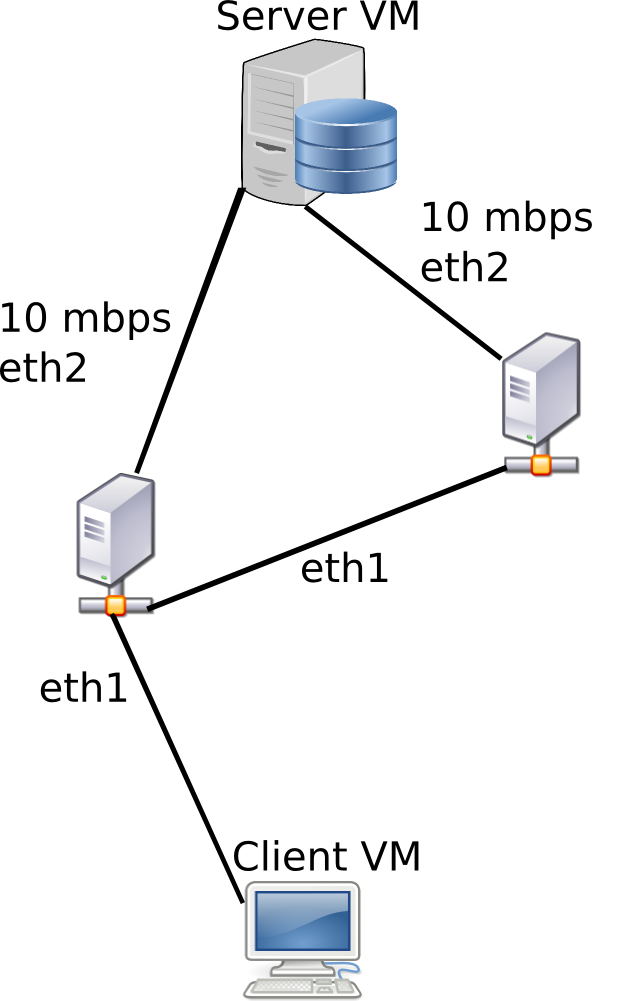
\includegraphics[keepaspectratio=true,scale=0.3]{InterfaceSetup.png}
		\caption{VM diagram}
		\label{fig:awesome_image}
	\end{figure}

	Initial evaluation results were satisfying. Our baseline case consisted of two routers, each with a $10 mbps$ throttled connection to the server, and an unthrottled (near instantaneous) connection with each other and their clients. Using a 40 Megabyte test file, downloaded in 1 Megabyte chunks, the total download speed (realized by the client) was close to being doubled, at $18 mbps$. A significantly smaller test file of $7 mb$ yielded speeds of $17.3 mbps$, suggesting that the small overhead induced by our aggregation techniques is diminished with larger file sizes. After extensive testing in our controlled virtualized environment, we found that the realized bandwidth of the client converged towards $90\%$ of the combined offered bandwidth of each router.

	\subsubsection{Effect of Chunk Size on Realized Bandwidth}
		Our algorithm for aggregating bandwidth works by segmentally downloading a target file in consecutive chunks of a fixed size. As the size of the chunk (relative to that of the file) directly determines the number of requests which must be sent to the server (then processed by the proxy), we sought to find a desirable chunk size which would accrue as little overhead as possible. Since our target environment (embedded Linux systems) have limited memory, we chose an upper bound of $32 mb$, as larger chunk sizes would quickly exhaust buffer space. Bandwidth gains increased logarithmically with respect to chunk size. However, gains actually shrank considerably when using chunk sizes larger then $5 mb$. 
		
		\begin{figure}[H]
			\centering
			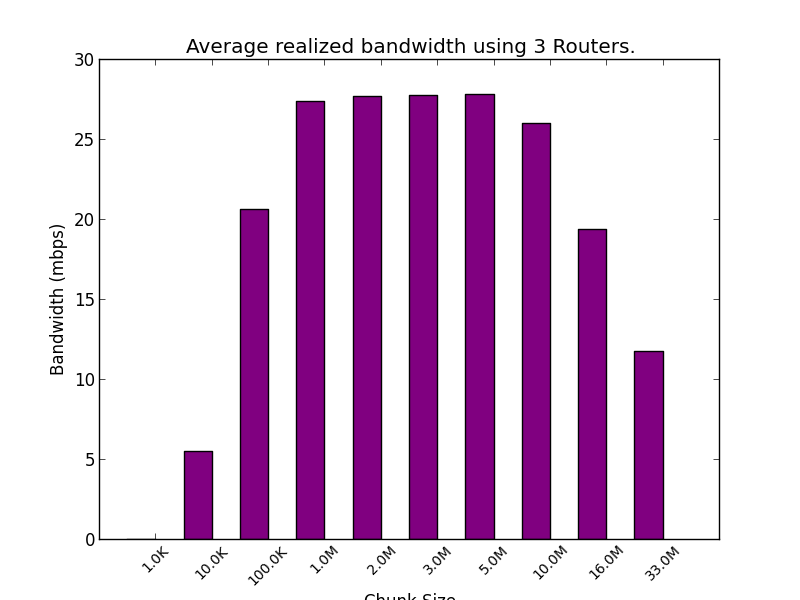
\includegraphics[keepaspectratio=true,scale=0.5]{all_sizes.png}
			\caption{Average bandwidth with respect to chunk size. Three routers were used, with their server connections fixed at $10 mbps$}
		\end{figure}

		On the opposite end of this spectrum, lies the invariably smaller chunk sizes (of less then $100 kb$). We found that chunk sizes below this limit yielded poor download times. The minimum tested chunk size used was $1 kb$, which produced results far less then the offered bandwidth of a single router, even when multiple routers were used in aggregation. For this chunk size, the realized bandwidth was a tenth of a percent of the offered bandwidth from the pool. Using $10 kb$, the damage was less worse, at $21.5\%$ of the offered bandwidth. Using $100 kb$ chunks produced a combined bandwidth that was $75\%$ of the theoretical offered bandwidth of the participating routers. For this reason, we concluded that a lower bound on chunk size of $100 kb$ was necessary in order for aggregation to become practical.

		Further investigation of the lower chunk ranges showed a steep logarithmic raise as chunk sizes grew from $1 kb$ to $1 mb$. Increasing the chunk size past $1 mb$ garners only fractional throughput gains, and presents a greater risk to buffer bloat. 

	After gathering conclusive data through our virtualized test suite, we conducted a brief proof of concept test using real hardware. We ran Ubuntuu 12.04 desktop on two PCs, each equipped with USB Wireless NICs. These dongles allowed us to mimic wireless inter-router communication, so that our real world tests came as close to mimicking the router environment as possible. Since we were limited to only two machines, each computer had to take on a double roll in the tests. Each acted as a router. One doubled as a client, the other doubled as our server. The latter ran a local instance of Apache, and used a special module to rate limit connections from each client to a specified throughput. This allowed us to enforce per-connection bandwidth constraints. 


\newpage
\section{Discussion}
	
	Devising a proper approach to bandwidth aggregation at the application layer spurs a plethora of discussions, some of which are unique in scope to this paper. As far as these authors are concerned, no existing works in the niche field of bandwidth aggregation take the issue of security as seriously as this MQP attempts to do. 
	\subsection{Rationale for various Design decisions (and their alternatives)}

		We identified a number of key design points involved with our software. This sections attempts to highlight both the naive and optimal way of approaching many of our design problems. As well as our rationale in choosing the ones we did. We note that the finished software implements the former in most cases, but could be extended to achieve the optimal approach for each design case. 

		\subsubsection{Packet Segmentation Algorithm}

			We first devised a na\"{i}ve approach to splitting up the work for a particular file, which works as follows. Given a peer network of $n$ routers, give each router: $$\frac{FILESIZE}{n} bytes\; of\; capacity$$. This has a major shortcoming however; different routers download at different rates, so the file download is not complete until the slowest router has downloaded and transmitted its chunk back to the host. The effective download time becomes a function of the download speed of the slowest router. A better approach is to divide up the file into chunks using a relation between individual router bandwidth and total pool bandwidth.

			A consideration to keep in mind is that the host router may not be directly connected to each available peer, and certain peers may be connected to each other better then the host router. It could be the case that the host has 3 peers, who each have 3 other peers in wireless communication range. When the router splits up these chunks, the advertised bandwidth of a router that he is directly connected too should reflect the average bandwidth of all of that routers peers. So if $A$ connects to $B$, who has $2 mbps$ of bandwidth, but $B$ can talk to $C$ and $D$, who each have a $10 mbps$ connection, $B$ could advertise to $A$ that his bandwidth is $$\frac{B + C + D}{3} mbps$$. This will help $A$ more accurately decide how to manage the file segmenting. When $B$ is passed this chunk, it can do the same with each peer in his network.

			The problem of overlapping neighbors does immediately become an issue. This would be addressed at the implementation level. The host could generate a random session key, and pass the key along when it communicates with its neighbors during the negotiation period. Each neighbor will store this key, and until a cancel request is sent from the host, the router will reject any negotiating requests whose key matches their stored key. This way, a router will not commit its bandwidth too two different neighbors on the same file download.

			Pseudo code of the algorithm:

			\begin{algorithmic}
				\ForAll{peer in neighbors(host)}
					\State $netBandwidth\gets netBandwidth + peer.bandwidth$
				\EndFor

				\ForAll{peer in neighbors(host)}
					\State $Chunk_{peer} \gets \frac{peer.bandwidth}{netBandwidth} \times{fileSize}$
				\EndFor

				\ForAll{peer in neighbors(host)}
					Delegate $Chunk_{peer}$
					\State $AmountRemaining \gets AmountRemaining - Chunk_{peer}$
				\EndFor\\
				Issue HTTP GET for $AmountRemaining$
			\end{algorithmic}

		\subsubsection{Boundaries on segment size}

			There are a number of pitfalls that this type of segmentation produces. When a file is downloaded in one session under normal conditions, the round trip time for the request (reaching the server, getting the first response) has a negligible impact. As TCP's AIMD pattern begins, an appropriate window size is established and transmission time smooths out. Fortunately, the TCP overhead can be avoided because HTTP 1.1 uses persistent TCP connections, so the setup only has to happen once for each peer, just as with a normal download.

			The round trip delay (RTT), while negligible for single session downloads, presents an issue when the download is broken into segments. The RTT overhead is applied to each segment request, for each peer. This gives the following relation:
			$$Overhead = \frac{file size}{segment size} * RTT$$
			The overhead grows as segment size decreases, so a larger segment is desirable. This presents a problem for devices with limited buffer space. For example, a typical home router will have anywhere between $1$ and $32MB$ of buffer space to spare. This is because the router has to buffer the request data in RAM, where its firmware (presumably OpenWRT, as well as our program) also resides. To use all the available buffer would result in buffer bloat (the excessive consumption of buffer space), leaving it with little room for other applications and ultimately leading to congestion at the link. As such, a fraction of the buffers total space should be used. It goes without saying, that we need to optimize for lower buffer consumption. This means that each router can only download a set amount at a time, and must wait until the client is ready to request more. This idle time should also be considered. Fortunately, the overhead is outweighed by the gains of downloading in parallel, especially when multiple peers are involved.

			In our implementation, we used the na\"{i}ve approach, and aimed for smaller chunk sizes, that could be held in a queue on the coordinating router without using an excessive amount of RAM. One might imagine a target resource as an array of contiguous, fixed length chunks, which are allocated to peer helpers on a first come, first served basis. These chunks are written back to the client, in order, as they come in.

	\subsection{Security Goals}

		The biggest problem with our approach to bandwidth aggregation, is that it puts the end client in control. Our chief concerns are data integrity and download liability. The former can be achieved through an implementation of the zero knowledge protocol, the latter is addressed by asymmetric cryptography. In addition, the goals of availability and confidentiality will be considered. Availability is by far the most important factor, as a disabled router will certainly lead to quality of service concerns on the client end. It is one thing to guarantee a faster Internet connection, but to do so at the cost of service entirely is unacceptable. Confidentiality is certainly desirable, but difficult to achieve in our case, as the operator of a peer's router has the right and power to view any traffic allocated to it. From a security standpoint, any peer can be thought of as a required man in the middle, who's presence must be tolerated for the sake of the aggregation. 

		The easiest scenario to envision for accessibility issues is that of a denial of service, instigated by a peer. If a peer could simply demand bandwidth from its neighbors endlessly until they were no longer capable of serving their own clients, then accessibility is certainly breached. For this reason, peer routers volunteer at will to join aggregation sessions. If a client on a peer's network suddenly demands more bandwidth, the peer may opt out of the session, and the initiating router will react accordingly. The routers will listen on a shared TCP port, which any peer may close themselves if they wish to opt out of bandwidth aggregation (in either direction).

		Blindly accepting file data from a peer router would certainly be a huge security hole. As the data being sent back to the client is stored directly to their hard disk (presumably with the pretense of being accessed very soon) a corrupted or pernicious file in the guise of meaningful content could cause havoc on the compromised computer. In cryptography, the Zero Knowledge Proof\lcite{The RFC} is a technique in which two parties, a prover and a verifier, exchange and verify the truth of a piece of data without the use of external information. In the case of this MQP, the coordinator (the verifier) must check segment data coming back from each peer (the prover) for validity. To do so, the coordinator will choose a random section of bytes within the range of the segment range it asked the peer for. When the peer responds, it will check the response against the verify bytes that it downloaded its self, rejecting the response if the bytes don't match. A malicious peer has no way of knowing which segment the coordinator will check, so the possibility of being caught outweighs the small probability that the attacker correctly guesses the piece that the verifier will choose\footnote{With a segment size of 1000 bytes, and a verification size of 4 consecutive bytes, the probability of both the verifier and prover choosing the same sequence is $2.006\times10^{-9}$}.The peer has no choice but to send the legitimate segment. This is both a secure and easy to implement solution, with only a small degree of additional overhead. The RTT for each segment is now doubled, as two requests must be made to the server, but these requests would reuse the TCP connection already established with the server for normal chunk downloads, which mitigates the impact of the overhead. The overhead is certainly a concern, but can be alleviated by decreasing the rate of verification as peers become more trusted. The coordinator could dynamically back of and only check a few times per session. The potentially malicious peer still has no way of knowing if the coordinator will verify any given transaction, so the zero knowledge principle can be assumed here as well. 

		While our application of the Zero Knowledge protocol works well in theory, it makes two dangerous assumptions, namely, that the content being verified is static (at least within the window of verification), and that the server is truthful. The former issue may be overlooked, when one assumes that most large file downloads are static. But this assumption limits the application of our software to resources conforming to this type, a facetious endeavor by all accounts. Internet video streaming is a paragon of dynamic web content. Streaming sites, such as Netflix, determine an optimal video quality for each session, in a similar way to TCP's congestion control. This means that content downloaded before a quality increase is helpless to be verified after one. Now, we have an added level of complexity to the seemingly straightforward verification process given by the Zero Knowledge proof. To complicate things even more, we may consider the case where the host server is untruthful. Suppose the server is asked for byte range 200 through 205, but really returns bytes 205 through 210. The verifier would again mistakingly incriminate the prover, when in fact, the server had been the cause of error. For these reasons, the verifier can at best only speculate the truthfulness of the prover.

		\subsubsection{Trust Platform, and Reliability}

			``Trust is fuzzy since trust is imprecise and vague. Trust is dynamic since it is not stable and it changes as time goes by. Trust is also complex since different ways are possible for determining trust.''\lcite{Chang, E., Dillon, T., Hussain, F.K.: Trust and Reputation for Service-Oriented Environments.Wiley (2006)}. 

			It is important in our aggregation model, that participating routers have a well-founded trust established between each other. A peer that is caught sending virulent data should be subject to significantly more skepticism then a peer who has no violations. Similarly, a peer may not wish to involve its self in a session that an untrusted neighbor is initiating. A security trust relationship is needed, and it must be dynamic and responsive. Selecting peers with desirable resources (bandwidth) and trust can be achieved in a variety of ways. While in certain scenarios, a trusted third party could alleviate some or all of the pressure involving trust calculations, we are unable to make use of it. The trust model must be dynamic and self regulating. A reputation based model could be used, where peers seek information about the quality of past experiences other peers have had with a untrusted peer, evolving into a semi-complex who-trusts-who social network.

			The definition of trust: Trust is a quantified belief held by a peer, which is formed through the observations and recommendations, with respect to another peer’s ability to complete a particular task successfully. 

			The peer-to-peer (P2P) network model has all these demands. We looked to this field for answers and insights into how we might go about developing a trust model for my protocol. As it turns out, this is an open area of research in P2P, so there was a great collection of data to check over. One such model employs data-signing in order to verify how credible data coming back is. Peers who have more valid data-signatures are deemed more trust-worthy. This is a popular approach to trust in file sharing P2P applications. In larger P2P networks, a single client can not possibly interact with every other node itself in order to evaluate trust. This puts forth the need for a reputation based trust model, where a peer evaluates the trust level of another peer through the claims of other peers who have interacted with the peer in question. Xiong et al. identify a number of other concerning characteristics of the reputation model. For instance, if the feedback mechanism is not incentivized, then a peer being asked for information regarding its experience with another peer may simply lie, and poison the askers understanding of the peer in question. A peer may also discretely raise and lower trust by preforming many small transactions truthfully, in order to build sufficient trust to be involved in a larger session, which it may then lie about (a sting operation!)\lcite{Xiong PeerTrust}.

			Xiong et al. introduce an elaborate approach that attempts to fix most of the outlined problems with a reputation based model. This includes feedback scope, which adds a context of the feedback (was the interaction trivial or monumental), as well as credibility factor for each peer, which is used to asses the trustworthiness of a feedback provider\lcite{Xiong}. For our application, the reputation model may not be necessary. In a practical sense of our application, there will likely be a small number of peer nodes in a single wireless bandwidth pool. Further, since each peer is within a somewhat close proximity, and each peer is maintained by a real individual (the router owner), it is less likely that either a peer or its owner will never interact with another peer. In our case, the overhead and unreliability of the reputation model would not be worthwhile. Where we to do one, it would likely work as follows: at the end of an aggregation session, the coordinating peer would broadcast its peer feedback report to all peers involved in the session, so participants would gain a better understanding of other participants who they were not directly involved with. The benefit here is that a malicious peer can be identified immediately. However, the downside is that the coordinating peer has too much power. It can easily lie about any interaction it had.

			Accumulating trust through record keeping is a reliable method, but falls short because due to its slow start methodology\lcite{p2pTrustRecommendation}.Our bandwidth aggregation schema is more static, in that neighboring peers who involve themselves are likely to be in a relationship for a long time. A real world example to relate would be that of a new neighbor moving into an apartment complex. Suppose that some or all of the residents in this complex are using the bandwidth aggregation model described herein. If the new neighbor wishes to join in, the other routers will at first be wary, possibly choosing to include him in a only a subset of interactions. But once trust has been built, it will pervade until the peer performs a malicious action, or the peer`' router's owner moves away. Since new nodes are not continuously swapped in and out on a daily basis, a local trust model should suffice for our application.

			There trust calculations can be modeled mathematically. One approach, suggested by Medic et al., is to represent a peer's trust factor as a tuple of Trust and untrust. Mathematically $F = [T,U] $, where $T = Trust$, and $U = Untrust$. The benefit of this model is that differing weights can be assigned to each trust factor component. This simulates a weighted average of the two factors.\comment{not in the equation!}

			In our protocol, it may be the case that a peer who misbehaves in the past corrects themselves for all future interactions. Their past violation should only act as a brief hiccup, and not hurt their trust factor for the rest of their existence. This desire suggests a weighted average of each trust factor, between past and recent interactions. Past interactions would be weighed less heavily when computing a peer's trust factor, whereas recent (within the past 12 hours) would be assigned a heavier weight. This allows for a peer's trust to evolve with their actions, and scale off better recent behavior. Each trust value will be within the interval of [0,1]

			Borrowing from Xiong et al.'s approach to trust computation, we chose to store trust on a transaction level. Here, a transaction represents one download session held between a coordinator and a peer. The transaction will hold the computed trust factor for that session. If all goes well, the value will be [1,0]. However, if the peer made any untrustworthy actions, the second value (untrust) will be higher, resulting in a lower trust value. The trust factor metric is computed by the summation of each of these transactions (with a higher weight assigned to more recent transactions, good or bad). In their PeerTrust model, Xiong et al. model feedback that the coordinator has with peer $u$ from transaction $i$ as $S(u,i)$. We will use this normalized amount of satisfaction for the formation of our trust factor score. Note that $I(u)$ denotes the number of transactions the coordinator has had with peer $u$, $W(u,i)$ denotes the weight assigned to the feedback the coordinator has had with peer $u$ at transaction $i$ (based off the time of transaction), and $R(u,i)$ denotes the untrust feedback from transaction $i$ with peer $u$. With this information, $T(u)$ (trust) and $U(u)$ (untrust) are calculated as follows:
			$$
				T(u) = \frac{\sum\limits_{i=1}^{I(u)} S(u,i) * W(u,i)}{I(u)},
				U(u) = \frac{\sum\limits_{i=1}^{I(u)} S(u,i) * W(u,i)}{I(u)}
			$$

			Once the metric has been computed, the trust making logic is fairly simple. If $T(u) > U(u)$, then the peer is trustworthy. If not, the peer cannot be trusted. Since trust is just one of the many metrics that will go into peer selection, simply assessing trust on a binary level is sufficient. 

			Given this formula for averaging trust, we still must add one more vital component before a score can be derived, the trust value. In examining multiple papers on p2p trust analysis, we found a number of terms and considerations that need be introduced. With unforgeable identities (in our case, private keys generated by a trusted central source), it should be difficult for a peer to erase their given identity (and reputation associated with it) and begin anew with a fresh identity. Such a peer could use this technique, known as whitewashing, in order to rebuild their reputation. This is an issue in systems where new peers are trusted from the start.

			Stakhanova et al. present a through outline of Trust information, in terms of what is gathered and how it is scored. The transaction quality can be modeled as positive, negative, or a combination of both. They note that a versatile will consider both, as relying on only negative feedback can may lead to wrongful elimination, while relying on only positive can allow malicious peers to fake benevolence. Second, the size of the files exchanged can also play a role.\lcite{Stakhanova}

			Trustworthiness can be modeled in multiple ways, where the chosen method is entirely dependent on the needs of the system. Some P2P systems, such as XREP and Travos, store trust as a binary value, meaning that the transaction was or wasn't satisfactory. The converse approach is to model trust as a discrete value on the scale of [0,1], allowing for partial trust to be modeled\lcite{Stakhanova}. In many systems, it is important to record the time of the interaction. This allows recency to be factored into trust decision making, like giving less weight to older values.

			Different approaches to transaction storage will yield different trust values. The memory efficient approach would be to store one average record, and update each component on a per transaciton basis. This has great appeal on devices with low memory (such as routers), but it sacrifices the elements of recency that help contribute to a more accurate understanding of the peer's trust. However, storage requirements in this scenario increase linearly over time as the number of peers in the system grow.

			Stakhanova et al. note that in cases where a few well known peers interact with each other often, storing trust locally is sufficient for each of them to make decisions. This obvioulsy doesn't scale for applications with millions of participants. This project will adopt the former approach, as the number of involved peers are limited to a finite local wireless range, which wouldn't typically exceed more then a dozen peers\lcite{Stakhanova}.

			How do we compute the actual trust calculation? The smallest scale we can start on, is at the per-chunk level. Selcuk et al present a solution that uses a bit-vector of m interactions. The bits are either 1 or 0, when the data is authentic or inauthentic, respectively. For our project, each peer has a chance to verify every chunk that is sent. The bit vector could hold $m$ bits, where $m$ is the number of chunks verified. As trust grew, $m$ could become smaller and smaller, reducing the verification overhead. The overal trust from a transaction is computed by treating the $m$ significant bits in the vector as a signed integer\lcite{Selcuk}.
				$$
						\frac{m-bit vector}{2^m}
				$$
			Dividing by $2^m$ produces a score on the interval of [0,1). This score can then be stored in the transaction record, and used in the averaging function mentioned above. The benefit of the system is that it accumulates a continuous trust value from many binary transactions. When a file is verified, it either passes verification or fails. Selcuk et al also provide a formula for calculating the inverse of the trust value, distrust. The method is the same as with trust, except that the m-bit vector is inverted (isolating the failure cases). During a download session, a running value of the distrust could be kept, so that once a certain threshold is reached, the malicious peer can be dropped. An isolated distrust value allows us to apply our own weight to distrust, so that a inauthentic response can be weighed more heavily. 




		\subsubsection{Responsibility with Asymmetric Cryptography}

			Since bandwidth aggregation is often used as a means to accelerate download speeds for large files, some considerations regarding these very types of files arise. Large files can be many things, such as a computer application, a compressed music library, or video data. All these cases are susceptible to copy right infringement due to illegal download. This scenario introduces a key problem concerning each peer. If a client wishes to download copyrighted material illegally, and aggregation is used, each peer router's owner is liable for the infringement, not just the client. This is explained in the legality section of this paper. Since it is impossible for each peer to asses the legality of a file being downloaded, there is little that a peer can do to prevent themselves from incriminating their clients (the network owners). 

			If a peer router maintained a log of each session that it participated in, which could definitively map each request made back to the coordinating host, then the peer could deny their liability in the implication, at least to some extent.\footnote{As no such case of copyright infringement by one party using multiple routers has occurred, there is no precedent to cite, so the outcome of such a trail is difficult to predict.}. If the log file could be falsified or changed, then it wouldn't hold up very well. Thankfully, asymmetric cryptography provides a way to map each request back to its originator: . Commonly referred to as public key cryptography, this cryptographic algorithm works by using two keys or signatures to encrypt or decrypt a piece of data. One key is made public, while the other is kept private. These two keys are intimately tied to each other. If the private key is used to encrypt a piece of data, only the associated key can decrypt it. Conversely, if the public key is used to encrypt, only the private key can decrypt. The former allows a piece of data to be definitively tied to the owner of the public key that decrypts it. If the decryption fails, then the message was not encrypted by the owner associated with the public key. In the latter situation, when the public key is used to encrypt, then only the owner of the associated private key may decrypt, so one and only one person can read the data.

			Implementing a fair non-repudiation protocol usually requires the presence of a trusted third party (TTP)\lcite{Zhou et al.}. It's involvement can range from frequent to sparing, being required for every request, or less then once per session. The extra communication and computational overhead caused by a TTP are hard to ignore. Its involvement can introduce a bottle neck in communication, and its trustworthiness is difficult to calculate\lcite{Kremer et al}. A TTP that involves its self in every interaction between Alice and Bob for a given message exchange is said to be inline. An online TTP only has to intervene a single time per exchange, avoiding unneccesary communication. A TTP is said to be offline if its involvement in a session is conditional\lcite{Kremer et al.}. An overview of some notable TTP based non-repudiation protocol proposals follows. 

			Zhang et al. devised a system in which the TTP broadcasts session information assigned to each message exchange to a publicly accessible board or web page. In our scope, the TTP could be any other router, and it could publish the session information to a central server which stores the information. The downside is that the records must be stored indefinitely, so the disk space will grow indefinitely\lcite{Zhang}.

			Zhou et al. propose a non-repudiation protocol which uses an online TTP to complete the non-repudiation process. The message exchanged between Alice and Bob is split into two parts; a key $K$, generated by Alice which is sent to the third party, and a commitment $C$ (produced by encrypting a message $M$ with $K$). The protocol begins with Alice generating $K$ and a session label $L$. The non-repudiation or origin and receipt messages are produced by signing a concatenation of the receiving router's IP, $L$, and $C$ with the senders private key . The protocol begins with Alice, who must generate both $K$ and $L$. She then sends her non-repudiation of origin message to Bob, who then replies with his non-repudiation of receipt message. Bob cannot read $M$ without first retrieving $K$ from the TTP. Alice then sends $K$,$L$,and the IP of Bob, encrypted with her private key, to the TTP. The TTP decrypts this 3-tuple and logs the information to a publicly accessible place, affirming Alice's proof of submission of $K$. Next, both Alice and Bob request a confirmation of $K$. This is the combination of both Alice and Bobs IPs, $K$, and $L$, encrypted with the TTP's private key. Alice simply logs this information, and Bob uses the retrieved key $K$ to finally decrypt the original commitment $C$, producing the message $M$\lcite{Zhou and Gollmann}.

			In this case, when Alice attempts to dispute sending a message to Bob, Bob will be able to prove she is lying, provided he has the information from above. A judge would have to examine the confirmation of $K$ sent by the TTP, as well as the non-repudiation of origin message originally sent to Bob by Alice. The one case that this fails is when Alice claims that her key was compromised, and that the signature on all of her messages was used by someone else\lcite{Zhou and Gollmann}.

			The integrity of the key pairs used for signing and verifying a message is of utmost importance. If a key is compromised, a non-repudiation protocol must be able to determine whether a signature was generated before or after they key was compromised. The straightforward approach would have Alice and Bob include a timestamp in their exchange, acting as evidence of the date of the interaction. Booth points out the issues with traditional public key encryption when used with time-stamps for non-repudiation.
			\begin{quote}
				if $A$'s secret key is suspect, it makes no sense to rely upon a timestamp which has been included in a message whose authenticity is attested to by that key. Any malicious agent (possibly $B$ or even $A$ himself) could easily concoct, timestamp, and sign such a message at any time after the supposed compromise and no one would be the wiser.\lcite{Booth}
			\end{quote}

			Booth proposes a TTP who acts as a notarizing agent. The TTP, acting as an authenticator, will append their copy of the sender's public key to the message, and sign it with their own. This practice is similar to that of a Notary-Public. Popek et al. proposed a similar system which also incorporates timestamps into the notarizing agent's contribution. Here, Alice first sends her signed message to a notary TTP who adds a timestamp and then encrypts the message with their own signature. Alice appends the relevant information (about the Notary whose private key was used to encrypt the message), and sends it to Bob\lcite{Popek et al.}. They point out that while using a single TTP as a notary adds substantial resilience to denial arising from compromised keys, the system can be exponentially enhanced with the addition of more notaries for each request.

			In the case of a compromised or revoked key, the time-stamp of a particular exchange must simply be compared to the date of revocation in order to verify whether the signing key was strictly private at the time of the interaction. We could modify the fair non-repudiation protocol devised by Zhou et al. to include this measure. The TTP could time stamp each interaction it coordinates, storing the time $T$ along with the session key and commitment message. When Alice and Bob retrieve the key for their own purposes, $T$ would be included so that all parties have a copy of the time stamp. In situations where a dispute arises, the Judge can simply compare the timestamp to the last known instance of the compromised key's validity.

			For our protocol, every peer could distribute their public key to each neighboring peer. The RSA cryptosystem could then be used for signing and verifying the message data. The sending peer would hash the original message, then sign the hash using their private key, and the RSA encryption method, and attach the computed hash as a HTTP header in the request. Each peer who receives the request simply has to match the sender's IP to their public key, and use it to verify the signature. This signature information could be logged to a file, along with IP, time stamp, port, and URL requested and used in all subsequent HTTP headers, so that the originators identity is preserved. The pycrypto library provides all the necessary functions to accomplish this.

			For a trial prototype, storing a text file of the IP to public key mapping is sufficient. For full scale deployment however, this fails to suffice. 

		\subsubsection{Peer selection by a variety of metrics}

			So far we have discussed a few ways to evaluate and choose between peers. The decision is not one to one, a coordinator must asses a given peer by a variety of metrics. These include estimated bandwidth, connection strength/reliability, and trust factor. But there exists a balance between speed and security. Certainly, a peer that is well trusted and has a high estimated bandwidth would be a good candidate for an aggregation session, but the two factors might not always balance. The coordinating peer must decide between a fast peer who is untrusted, and a slow peer who is well trusted. Although the goal of bandwidth aggregation is speed, we cannot ignore the inherent need for a secure system. So in the aforementioned scenario, an untrusted peer would not be picked.

			Reliability is another factor that will influence peer selection. Peers will be monitored for timeouts. If a peer fails to response to a resource request within a dynamically computed threshold (expressed as a worst case download time), the peer will be dropped for the session. After the session is ended, the number of timeouts the coordinator experienced with that peer will be recorded. 

			Network reliability is not a new field. There are a plethora of metrics we could use for our evaluation, but we are only concerned with a small subset of them. A ``reliable'' peer is one that transmits correct data in a quick and responsive manner. The first of these is channel capacity, a measurement of the number of bits that can be transmitted across a channel in a unit of time. This roughly corresponds to bits per second. 



\newpage
\section{Related Work}

		%TODO [Refactor]: Move this discussion to the Mobile Devices as An Aggregation Platform Section, and expand a little bit.%
		AT\&T Mobility li LLC holds a patent that applies similar strategies used in this MQP to aggregate WWAN clients who each have a static bandwidth allowance that is rarely in use. At a high level, the patent discusses a strikingly similar approach as this MQP, but is expressed strictly in terms of WWAN. Since this project aims to aggregate WLAN bandwidth, it is not a realization of the invention defined in patent no US7720098 B1 \lcite{Patent US7720098}.
		
		Octopus+ is a daemon that allows a computer with multiple means of accessing the Internet to dynamically combine the potential links to increase speed. This is most likely a round robin approach between the same Internet connections, and the product doesn't do any request splitting. It does gracefully handle link failures and selects the best link for each packet.
		
		% TODO: add citations for the commercial offerings
		There are also a number of commercial services that aim to bring bandwidth aggregation to the home. Multipath Networks offers an all in one aggregating router which uses Multipath TCP. They have a cloud infrastructure which handles reordering and aggregate traffic between any wifi, 3G, or 4G link. Telefonica, a Brazilian broadband and telecommunications provider, has been researching and developing a wireless aggregation solution, BeWifi, which claims to double bandwidth speeds for its customers. They follow a peer-to-peer philosophy, and construct a mesh network of cooperating routers in close proximity. Sleeping routers contribute their unused bandwidth to demanding neighbors, allowing potential bandwidth to be highly utilized at all times. Currently, they require a modified router to be installed by a technician, but hope to one day deploy a plug and play software upgrade. As this is a closely guarded commercial implementation, their research on the matter is all private. They note that fairness and security are a priority in their software, but fail to detail any of the underlying mechanism involved. They also fail to outline any counter measures in place to enforce repudiation between clients. 
		
		Many load balancing router's (D-Link DI-LB604, FatPipe XTREME, AstroCom PowerLink Pro) have been created, targeting both home users and enterprise businesses. These typically work by combining multiple links into a single one. 




\newpage
\section{Conclusion, Future work}


\newpage
\section{References}


\end{document}